% !TeX root = ../tg.tex
\chapter{基于分割-联邦学习的鲁棒性算法}
为了解决 SFL 中的标签噪声问题，我们在 SFL-V2 的基础上提出了 SFL-DCT 算法。SFL-DCT 受文献 \cite{b9} 中一种应对联邦学习（FL）中标签噪声算法FedCorr的启发。与已有工作不同的是，我们联合处理了分割-联邦学习中的非独立同分布（non-IID）数据和标签噪声问题，通过利用分割-联邦学习中服务器端可用的标签信息，并结合基于熵的思想来进行噪声检测。

为了评估 SFL-DCT 在实际场景中的性能，我们搭建了一个实验测试平台来实现该算法，这需要精心设计（例如并行传输、高效的内存与 CPU 使用），以减少训练延迟。接下来，我们将首先介绍算法的具体细节,然后介绍实验测试平台的设计。
\section{算法设计}
\begin{algorithm}[t]
\caption{SFL-DCT 算法}\label{alg1}
\begin{algorithmic}[1]
\STATE 初始化全局模型 $\omegab=(\omegabc,\omegabs)$ 和本地模型 $(\omegab_n, n\in\N)$，其中 $\omegab_n = (\omegabcn, \omegabs)$；
\STATE \underline{// \textit{第一阶段：噪声检测}}
% \STATE $avg(d)\leftarrow \sum_{n\in\N} d_n$
\STATE 根据 \eqref{calculate dn} 计算每个客户端 $n$ 的系数 $\gamma_n$；
\IF{$\max_{n\in \mathcal{N}} \{\gamma_n\} > \tau$}
\STATE 根据 \eqref{eq:LE} 计算每个客户端 $n$ 的 $\text{LE}_n$；
\STATE 基于所有 $n\in\N$ 的 $\text{LE}_{n}$，使用高斯混合模型（GMM）识别出干净客户端集合 $\N_{cle}$ 与含噪客户端集合 $\N_{noi}$；
\ELSE
\STATE $\omegab\leftarrow$ 所有客户端使用其数据集 $\mathcal{D}_n$，按照第 \ref{subsec:training} 节中步骤 1--4 进行 $R_0$ 轮 SFL 训练；
\STATE 根据 \eqref{definition of lid} 计算每个客户端 $n$ 的 $\text{LID}_n$；
\STATE 基于所有 $n\in\N$ 的 $\text{LID}_{n}$，使用 GMM 识别出干净客户端集合 $\N_{cle}$ 与含噪客户端集合 $\N_{noi}$；
\ENDIF
\STATE $\omegab\leftarrow$ 所有客户端 $n\in\N$ 使用其数据集 $\mathcal{D}_n$，按照第 \ref{subsec:training} 节中步骤 1--4 继续进行 SFL 训练，直到完成 $R_1$ 轮；
\STATE \underline{// \textit{第二阶段：噪声修正}}
\STATE $\omegab\leftarrow$ 干净客户端集合 $\mathcal{N}_{cle}$ 使用其数据集 $\mathcal{D}_n$，按照第 \ref{subsec:training} 节中步骤 1--4 进行 $R_2$ 轮 SFL 训练；
\STATE $loss_{n,i} \leftarrow$ 每个客户端 $n$ 中每条数据 $i$ 的测试损失；
\FOR{每个客户端 $n \in \N_{noi}$}
\STATE $\Dnoih_n\leftarrow$ 对所有 $i$ 上的 $loss_{n,i}$ 使用 GMM 进行分类，识别出含噪数据集合；
\FOR{每个 $(x_i,\tilde{y}_i)\in\Dnoih_n$}
\STATE 客户端 $n$ 计算 $h(x_i;\omegabcn)$ 并将 smashed data 发送给训练服务器；
\STATE 训练服务器计算 $h(x_i;\omegab_n)$，并基于输出 $h\left(x_i;\omegab_n \right)$ 修正标签 $\tilde{y}_i$；
\ENDFOR
\ENDFOR
\STATE \underline{// \textit{第三阶段：SFL 训练}}
\STATE $\omegab\leftarrow$ 所有客户端 $n\in\mathcal{N}$ 使用更新后的数据集 $\mathcal{D}_n'$（已完成标签噪声修正）按照第 \ref{subsec:training} 节中步骤 1--4 进行 $R_3$ 轮 SFL 训练；
\RETURN $\omegab$.
\end{algorithmic}
\end{algorithm}

SFL-DCT 的核心思想是先检测再修正标签噪声。该算法包含三个阶段：

- \textbf{第一阶段：} 使用本地内在维度（LID）检测独立同分布数据中的含噪客户端，使用标签熵（LE）检测非独立同分布数据中的含噪客户端。
- \textbf{第二阶段：} 利用来自干净客户端的数据训练全局模型，然后检测并修正来自含噪客户端的错误标签。
- \textbf{第三阶段：} 在修正后的数据样本上进行传统的 SFL 训练。

为便于表述，我们使用 $\omegab$ 表示需要训练的全局模型，并省略训练轮次的索引。需要注意的是，每个阶段（特别是第二或第三阶段）所使用的初始全局模型是前一阶段训练完成的模型。我们用 $\D_{n}$ 表示客户端 $n$ 的原始数据集。在第二阶段中，部分含噪标签会被修正，从而得到客户端 $n$ 的更新数据集，记作 $\D_{n}'$。

SFL-DCT 算法的伪代码如 算法~\ref{alg1} 所示，图~\ref{fig:SFL-DCT} 展示了 SFL-DCT 的整体流程。

\begin{figure}[t]
\centering
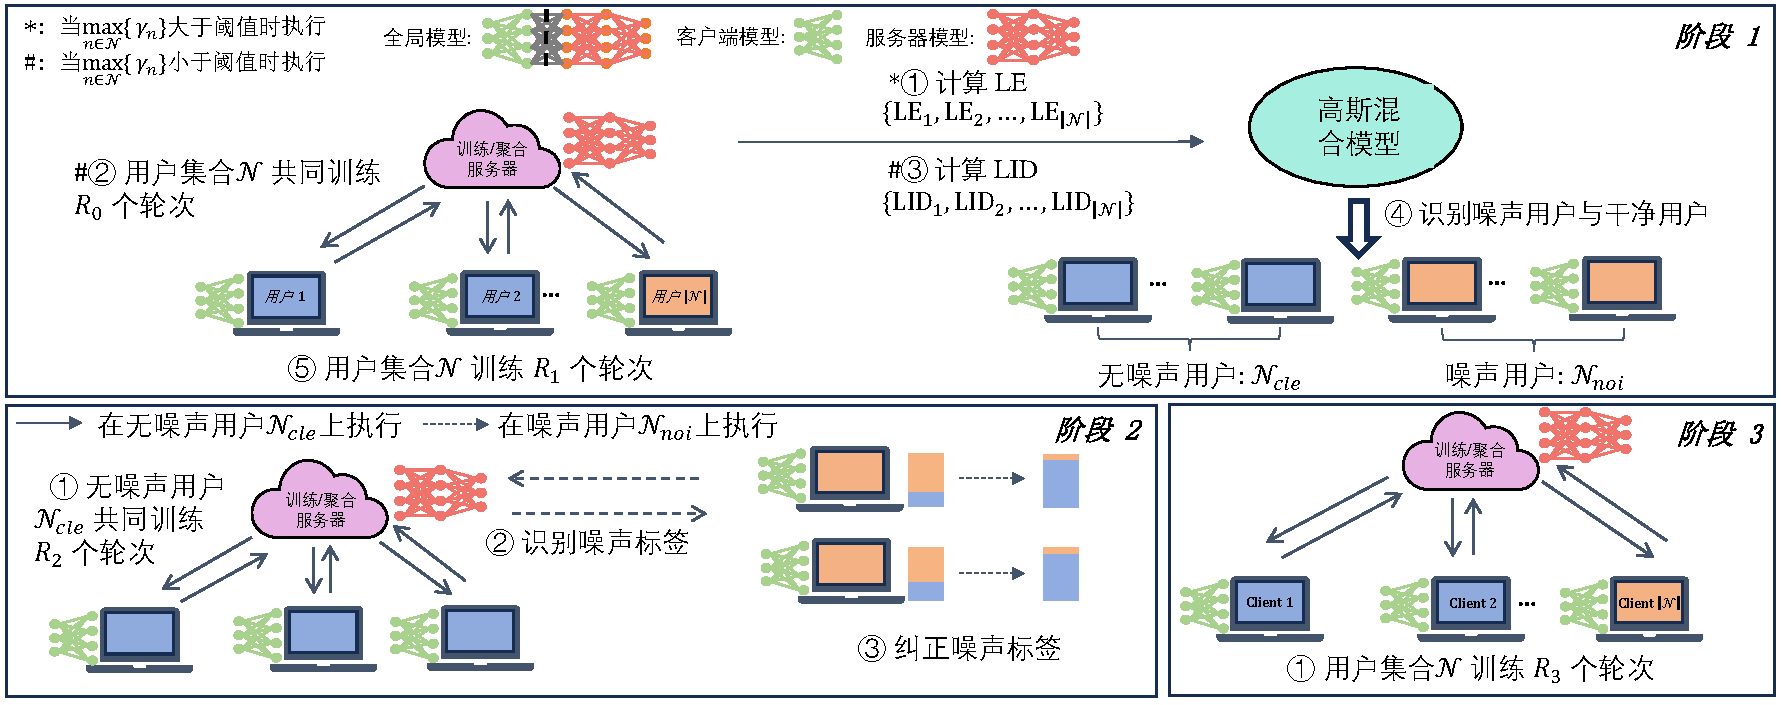
\includegraphics[width=\linewidth]{figures/al.pdf}
\caption{SFL-DCT 概览。}
\label{fig:SFL-DCT}
\end{figure}

\begin{figure}[t]
\centering
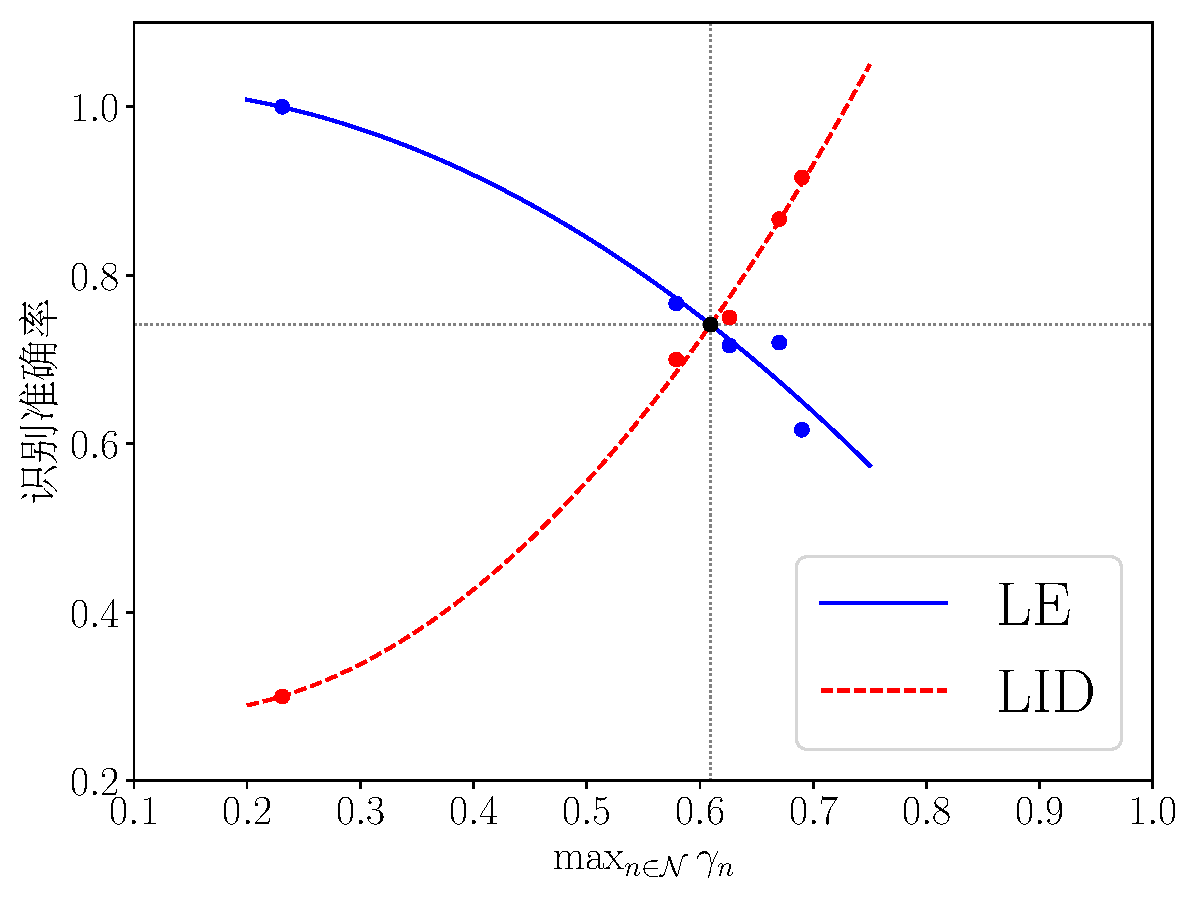
\includegraphics[height=5.3cm]{figures/gamma.pdf}
\caption{通过 LE 和 LID 方法检测含噪用户的准确率与 $\max_{n\in \mathcal{N}} \gamma_n$ 的关系。}
\label{fig:gamma}
\end{figure}

第一阶段的目标是检测存在标签噪声的客户端。在分割-联邦学习中，客户端会在训练过程中将标签发送给服务器 \cite{thapa2022splitfed,huang2023minibatch}。服务器为每个客户端 $n$ 计算一个系数 $\gamma_n$，用以反映该客户端数据集的非独立同分布（non-IID）程度。

为了计算 $\gamma_n$，服务器按升序排列客户端 $n$ 的标签频率。设 $(y_{(1)}^n, y_{(2)}^n, \dots, y_{(|\mathcal{K}|)}^n)$ 表示排序后的标签。

然后，$\gamma_n$ 通过计算前 $\lfloor K/{2}\rfloor$ 个标签所占数据样本的比例来确定：
\begin{equation}\label{calculate dn}
\gamma_n = \frac{\sum_{i=1}^{\lfloor K/{2}\rfloor} \text{count}(y_{(i)}^n)}{|\D_n|},
\end{equation}
其中 $\text{count}(y_{(i)}^n)$ 表示具有标签 $y_{(i)}^n$ 的数据样本数量。

根据所有 $n\in\N$ 的 $\gamma_n$ 值，我们选择合适的方法来检测含噪客户端。有两种候选方法：基于 LID 的检测和基于 LE 的检测。前者来源于文献 \cite{b9}，更适合 IID 数据集场景；后者则更适用于 non-IID 数据集。我们建议使用 $\max_{n\in \mathcal{N}} \gamma_n$ 来判断是否存在数据集极度非 IID 的客户端（即仅包含有限种类的标签）。如果 $\max_{n \in \mathcal{N}} \gamma_n > \tau$，则优先采用基于 LE 的方法；否则推荐使用基于 LID 的方法。其中，$\tau$ 是一个可以通过实验经验确定的阈值。

以 CIFAR-10 数据集为例，图~\ref{fig:gamma} 中的两条曲线展示了在不同 $\max_{n \in \mathcal{N}} \gamma_n$ 值下，LE 和 LID 方法检测含噪客户端的准确率。这两条曲线的交点表示最优的 $\tau$ 值，在该点上两种方法的性能达到平衡。对于这两种方法，训练服务器会通过计算每个客户端的 LID 分数或 LE 分数来评估其是否含有标签噪声。

\textbf{LID 分数：} 为了计算客户端的 LID 分数，首先让客户端使用 SFL 对全局模型进行 $R_0$ 轮训练。根据训练输出，对每个数据点 $(x_i,\tilde{y}_i)$，其 LID 定义如下 \cite{b9,amsaleg2015estimating,houle2013dimensionality}：
\begin{align}\label{eq:lid}
\text{LID}(x_i,\tilde{y}_i)=-\left(\frac{1}{k}\sum_{j=1}^k\log\frac{d_j\left(h\left(x_i,\omegab\right)\right)}{d_{max}\left(h\left(x_i,\omegab\right)\right)}\right)^{-1}.
\end{align}
在式 \eqref{eq:lid} 中，$d_j\left(h\left(x_i,\omegab\right)\right)$ 表示数据样本 $(x_i,\tilde{y}_i)$ 与其邻近样本 $(x_j,\tilde{y}_j)$ 在特征空间中的欧氏距离。考虑 $(x_i,\tilde{y}_i)$ 的 $k$ 个最近邻样本，即 $k$ 个具有最小 $d_j\left(h\left(x_i,\omegab\right)\right)$ 的样本。令 $d_{max}\left(h\left(x_i,\omegab\right)\right)$ 表示在这 $k$ 个最近邻中与 $(x_j,\tilde{y}_j)$ 的最大距离。

直观上讲，定义在 \eqref{eq:lid} 中的数据样本 LID 反映了该样本与其他样本的接近程度，从而间接揭示了其标签可能为噪声标签的可能性。每个客户端 $n$ 的 LID 分数为其数据集 $\mathcal{D}_n$ 中所有样本 LID 值的平均值：
% \begin{figure}[t]
% % \vspace{-15pt}
% \centering
% 
\includegraphics[height=3.3cm]{pic/demo.pdf} 
\includegraphics[height=3.3cm]{pic/time.pdf}\\
% (a)\qquad\qquad\qquad\qquad\qquad\qquad(b)
% % \vspace{-5pt}
% \caption{系统设计（a）与时间流程图（b）演示。}
% \label{fig:demo}
% % \vspace{-10pt}
% \end{figure}
\begin{equation}\label{definition of lid}
\textstyle \text{LID}_n = \sum_{(x_i,\tilde{y}_i)\in\D_{n}} \text{LID}(x_i,\tilde{y}_i)/|\D_n|.
\end{equation}

\textbf{LE 分数：} 我们提出使用标签的熵来衡量标签噪声。这一想法源于一个直观认识：随机噪声会使标签分布变得不那么集中。具体而言，LE 分数的计算方式如下：
\begin{equation}\label{eq:LE}
\text{LE}_n=-\gamma_n\log(\gamma_n)-(1-\gamma_n)\log(1-\gamma_n).
\end{equation}

随后，SFL-DCT 使用高斯混合模型（GMM）对 LID 或 LE 分数进行分类，从而区分干净客户端与含噪客户端。接着，SFL 训练过程继续进行，直到完成 $R_1$ 轮训练。需要注意的是，LID 的计算需要 $R_0$ 轮训练，而 LE 则不需要。进行至 $R_1$ 轮的训练确保了基于 LID 和基于 LE 的方法在相同训练水平上进行比较。

第二阶段通过使用被归类为干净的客户端（即 $n \in \mathcal{N}_{cle}$）来训练全局模型 $\omegab$，以提升模型准确率。训练损失用于识别每个含噪客户端 $n\in\mathcal{N}_{noi}$ 数据集中的噪声标签，因为噪声数据的损失通常较高。训练好的模型 $\omegab$ 随后被用于修正刚刚检测出的噪声标签。

在第三阶段，所有客户端 $n \in \mathcal{N}$ 在已修正第二阶段中检测出的噪声标签的数据集 $\mathcal{D}_n'$ 上继续进行训练，共进行 $R_3$ 轮。最终，获得优化后的全局模型。

\section{测试平台的实现}\label{sec:testbed}
\begin{figure}[t]
\centering
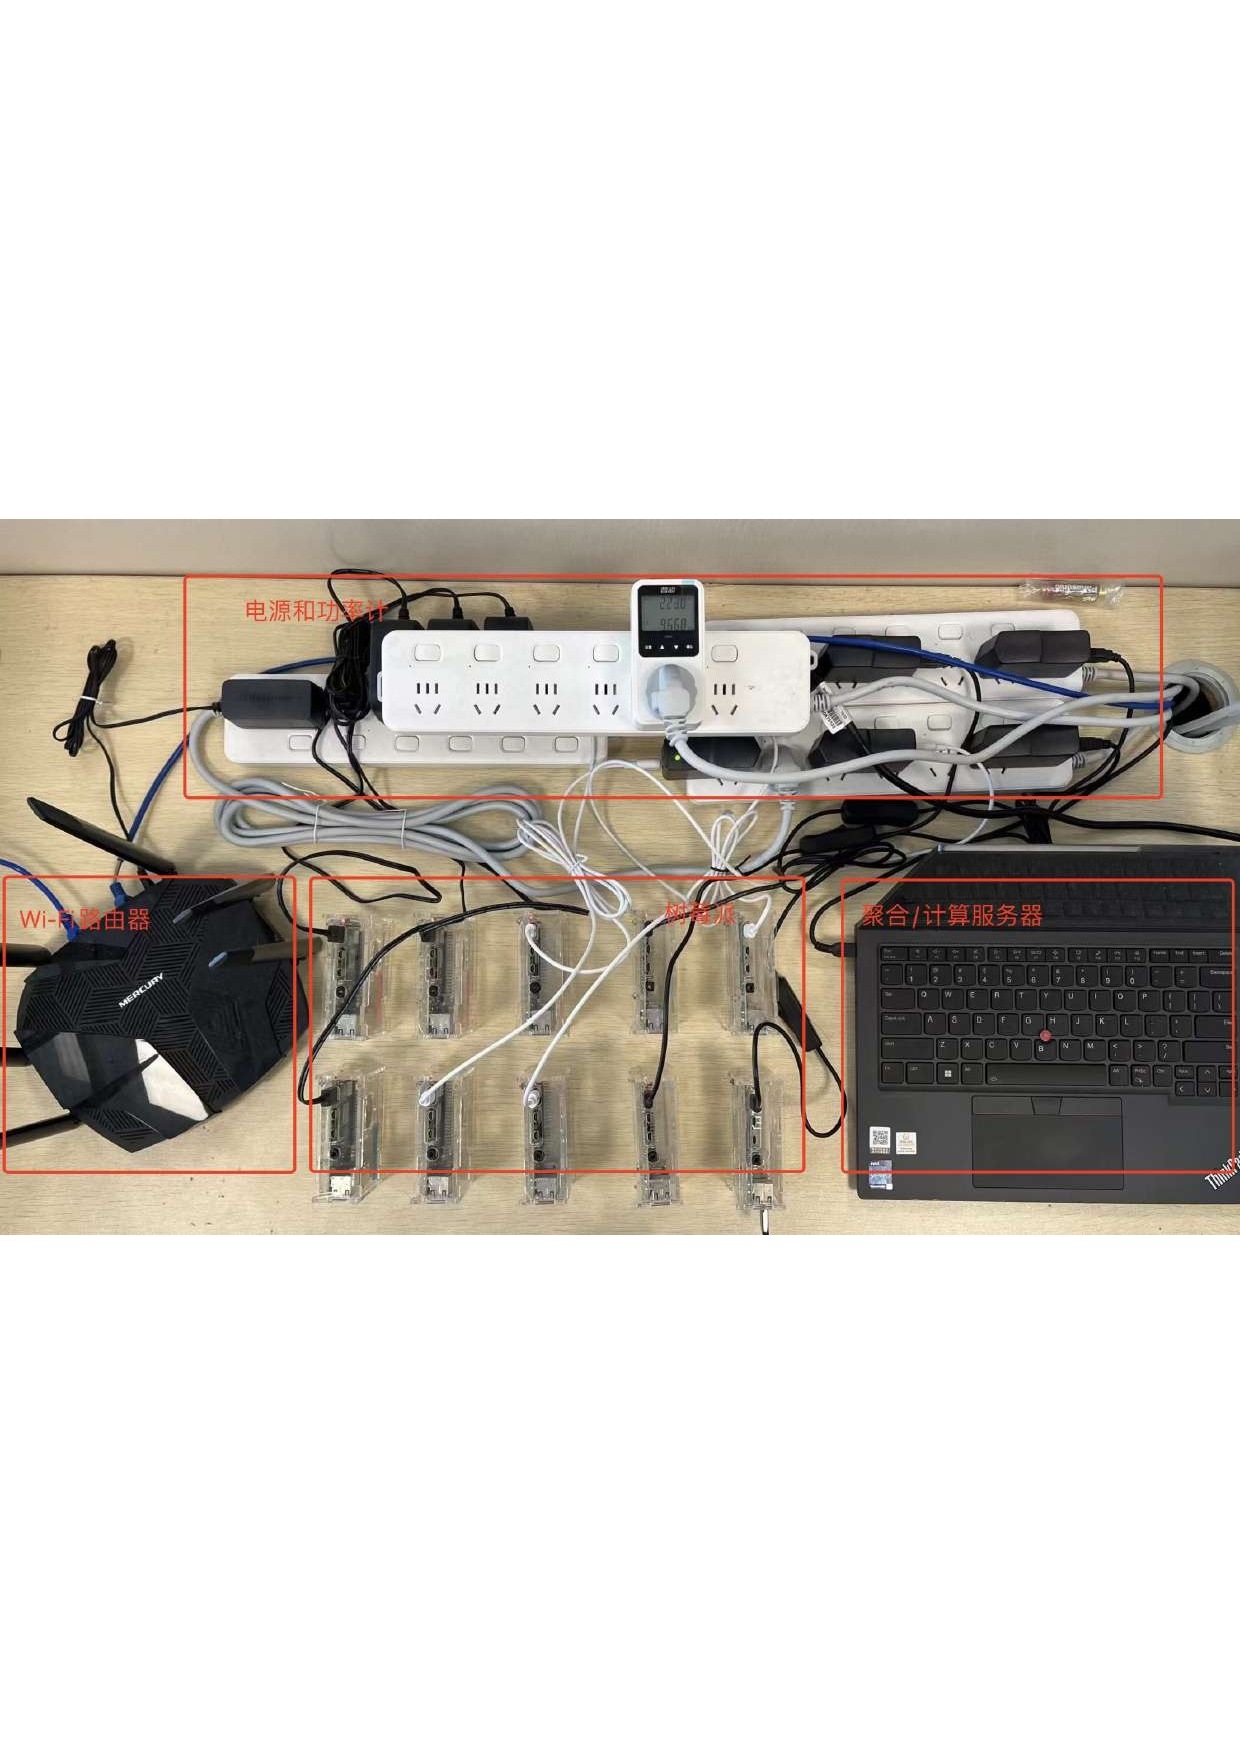
\includegraphics[height=3.5cm]{figures/testbed}
% \vspace{-5pt}
\caption{真实测试平台。}
\label{fig:testbed}
% \vspace{-15pt}
\end{figure}
在我们搭建的测试平台上，联邦服务器（fed server）和训练服务器（training server）部署在同一台个人电脑上（处理器为 13th Gen Intel(R) Core(TM) i7-13700K）。10个 Raspberry Pi 4B 设备作为客户端运行。由于 HTTP 协议具有较强的抗无线错误和丢包能力，我们在数据传输（如模型和梯度传输）中采用了 HTTP 协议。

每个客户端包含三个模块：客户端侧训练模块、HTTP 下载模块和客户端 HTTP 代理模块。服务器端则包括联邦服务器模块、训练服务器模块、HTTP 下载器模块以及 $N$ 个服务器端 HTTP 代理模块。HTTP 下载器与代理模块负责协调客户端与服务器之间的数据传输，同时支持并行数据交换（即双工通信，并允许多个客户端同时发送或接收数据）。

为了通过 HTTP 实现数据传输，每次数据传输都由一个 HTTP 请求触发。这种设计确保了数据交换的高效性与准确性，从而降低了分割-联邦学习的训练延迟，因为 HTTP 协议能够保证可靠的数据传输。
